\chapter{関連研究}
\label{chp:first}

\section{関連研究}
\label{sec:paragraph}
新しいマテリアルを使い,今までにない3Dプリンターでは表現できなかったモノを作ることを可能にしている研究を中心最新の3Dプリンターに関する研究を調査した.


\section{ゲルを用いて印刷する3Dプリンター\cite{a}}
\label{sec:enum}

この研究は,ゲルをマテリアルとして用いた造形物を3Dプリンディングするものである.
図1のように,ゲル溶液を使用しながら強度や感触を部位によって変化させて造形物を作成することができる.

\begin{figure}[H]
  \centering
  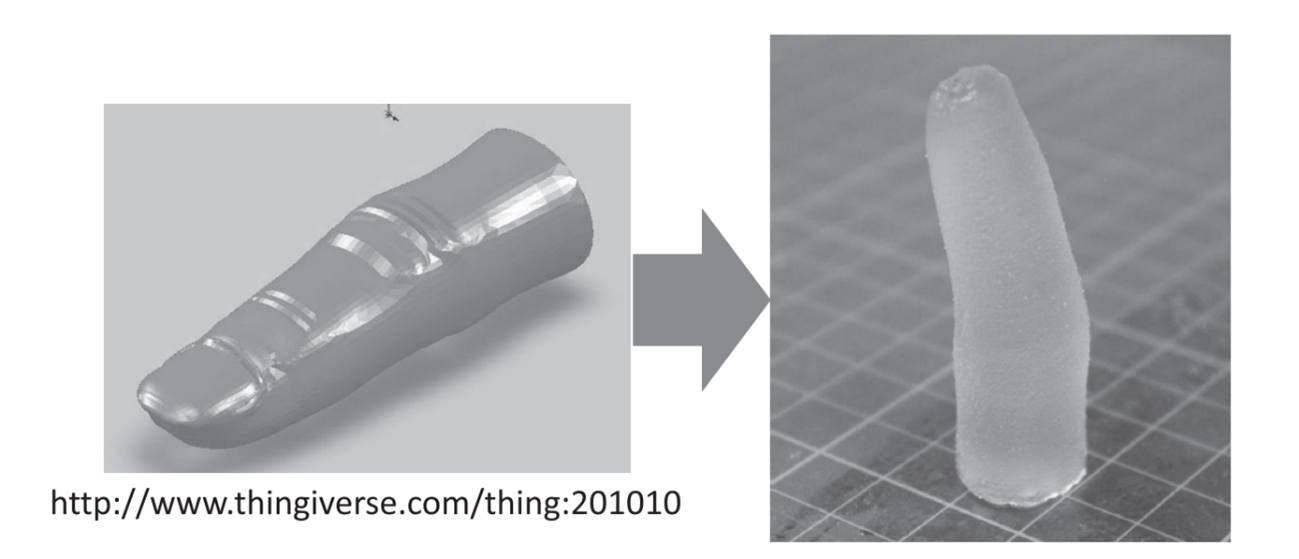
\includegraphics[width=6.4truecm]{./fig/ゲルを用いて印刷する3Dプリンター.png}
  \caption{適当なサンプル2}
% \url{http://www.this.is.sample.url/} % Web上のデータの場合、参照先URLを明記
  \label{fig:ゲル}
\end{figure}

これは,ゲル化を誘起するUVレーザーを光ファイバーを通して局所的にゲル溶液に照射することで,ゲルの3次元造形を可能にしている.3Dプリンターは現在,臓器の立体イメージを作り出すのに医療分野で活用されているが,手術の計画や事前検証のための立体の臓器モデルを作製するには,数千万もする工学な3Dプリンターを使用してプラスチックやゴムなどの,実際の臓器よりもはるかに硬い樹脂を用いて造形をする方法しか存在しなかった.
このゲルを用いて印刷する3Dプリンターは,低コストで感触がより患者のものと似ている臓器モデルを作成できる可能性を秘めている.

この3Dプリンターは材料として微粒子調整ダブルネットワークゲル(略称:P-DNゲル)を使用している.このゲルは強電解質性を示すモノマー由来の堅く脆い高分子ネットワーク(1st ネットワーク)と,中性を示すモノマー由来の柔軟な高分子ネットワーク(2nd ネットワーク)が相互侵入網目構造をとっている複合材料である.このP-DNゲル溶液にUVレーザーを照射することでラジカル反応が生じ,ゲルの3次元構造をつくることができる.


\section{Suntory-3D on the Rocks}
\label{sec:enum}

氷を掘削し様々な彫刻を作りお酒に入れて楽しむ試みがある.
多軸の CNC を使い掘削することで高精度の彫刻を作ることができるが,一般に普及させるのはコストならびに加工中の冷却の面から考えると難しい.

\begin{figure}[H]
  \centering
  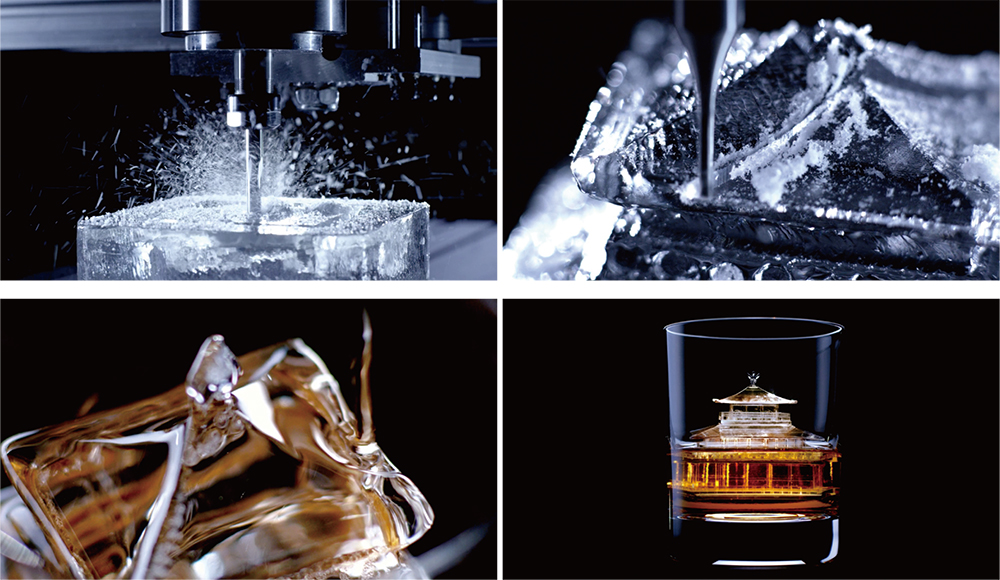
\includegraphics[width=6.4truecm]{./fig/Suntory.jpg}
  \caption{適当なサンプル2}
  \url{https://mag.sendenkaigi.com/brain/201406/up-to-works/002420.php} % Web上のデータの場合、参照先URLを明記
  \label{fig:Suntory}
\end{figure}


\section{A Layered Fabric 3D Printer for Soft Inter-active Objects}
\label{sec:enum}
この研究では布の造形物を印刷するためのプリンターを紹介している.
また,布の中に導電繊維の層を入れたり,コイル状の布を入れることで,タッチセンサーとしての利用法や NFC を使い LED を光らせるアプリケーションが紹介されている.
このプリンターの仕組みは,布のロールを引き出し天板に吸着させ固定し,レーザーでモデルの輪郭を切断し布のロールから切り出す.
この工程を繰り返し,アイロンの熱で接着していくことで造形物が完成する.

\begin{figure}[H]
  \centering
  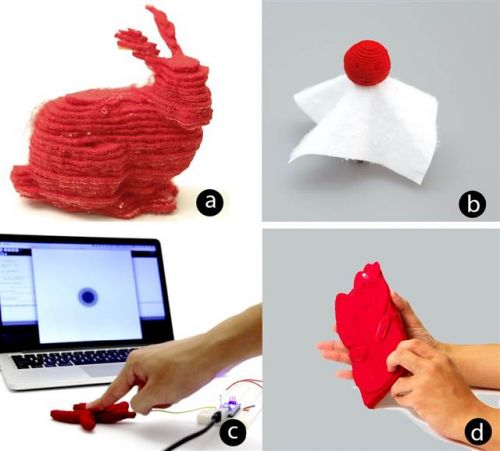
\includegraphics[width=6.4truecm]{./fig/ALayered.jpg}
  \caption{適当なサンプル2}
  \url{https://thelastnewspaper.com/a-layered-fabric-3d-printer-for-soft-interactive-objects/} % Web上のデータの場合、参照先URLを明記
  \label{fig:ferret}
\end{figure}



\section{ Additive manufacturing of optically trans-parent glass}
\label{sec:enum}
ガラスをマテリアルに使ったこの研究では,高温で流動性の高い状態に保持されたガラスを貯めておき,そのガラスを垂らすことで造形していく.
実際に造形されたガラスの造形物は一回のストロークで出せるラインは太く分厚いものであり,細かい造形はできないがサイズの大きい花瓶のようなものを造形することができる.
この手法で造形された花瓶は光を乱反射させる特性があり,上からライトを当て光の波紋を楽しむアプリケーションが提示されていた.


\begin{figure}[H]
  \centering
  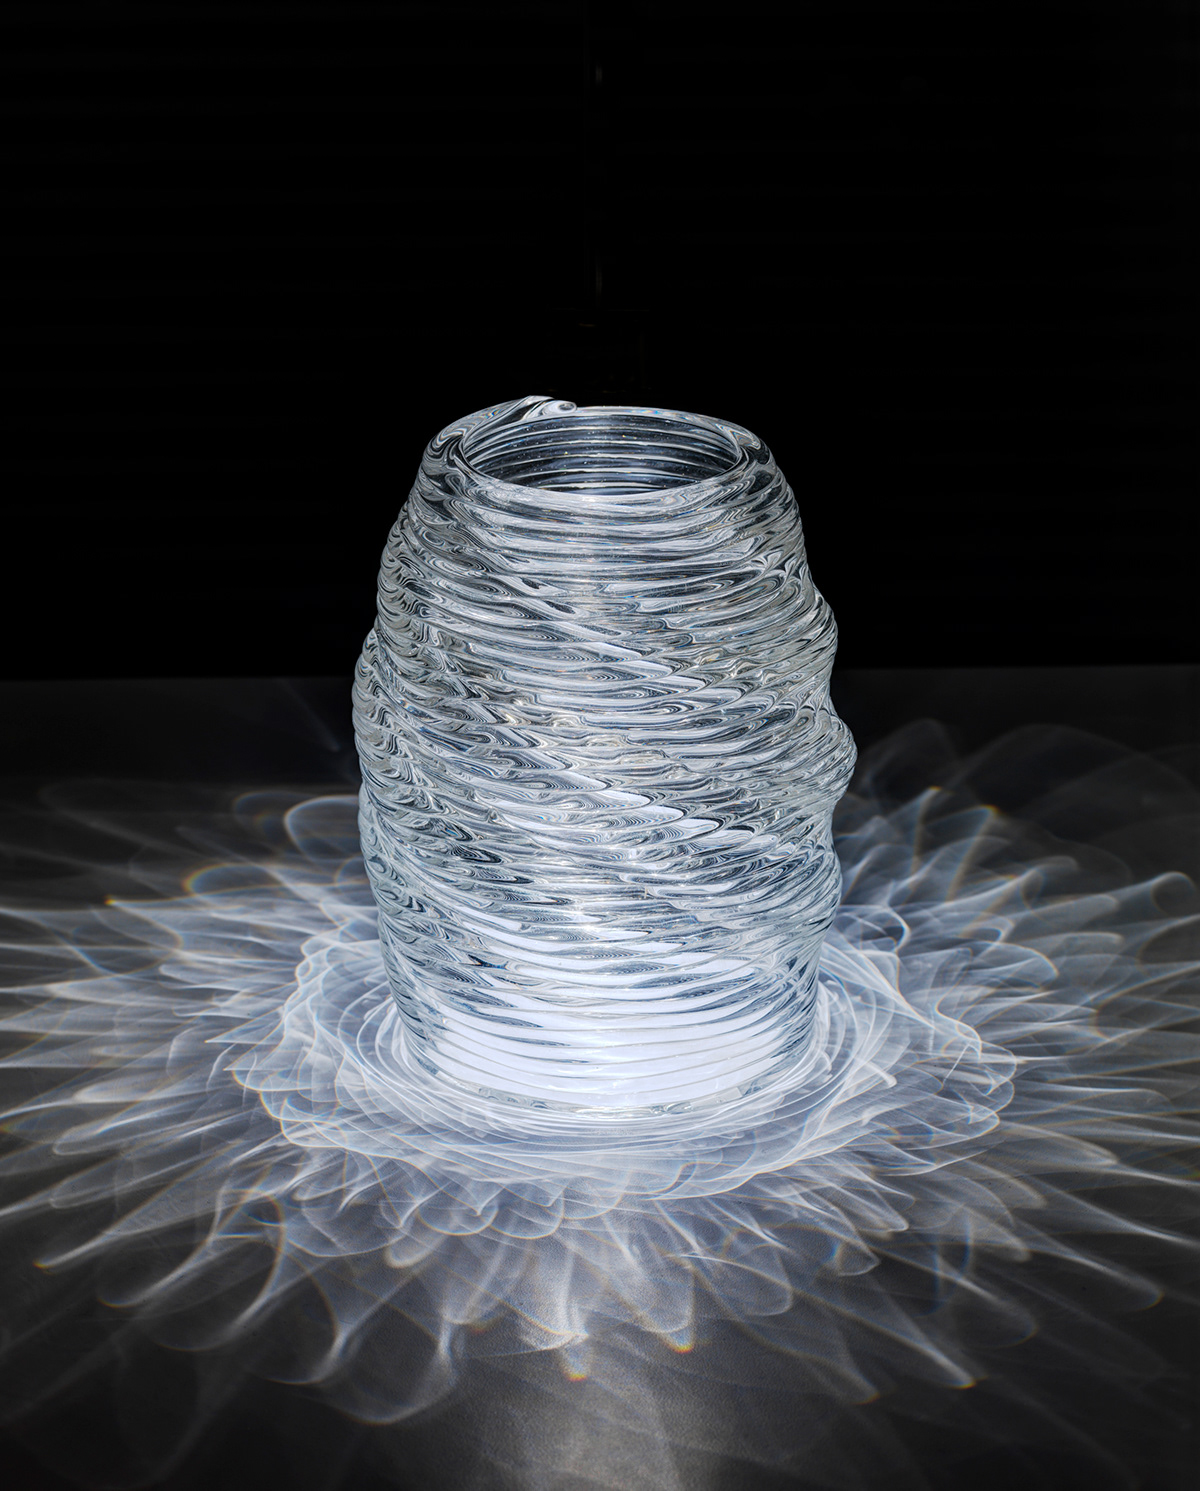
\includegraphics[width=6.4truecm]{./fig/Additive1.jpg}
  \caption{適当なサンプル2}
  \url{https://www.behance.net/gallery/65276297/GLASS-I} % Web上のデータの場合、参照先URLを明記
  \label{fig:ferret}
\end{figure}

\begin{figure}[H]
  \centering
  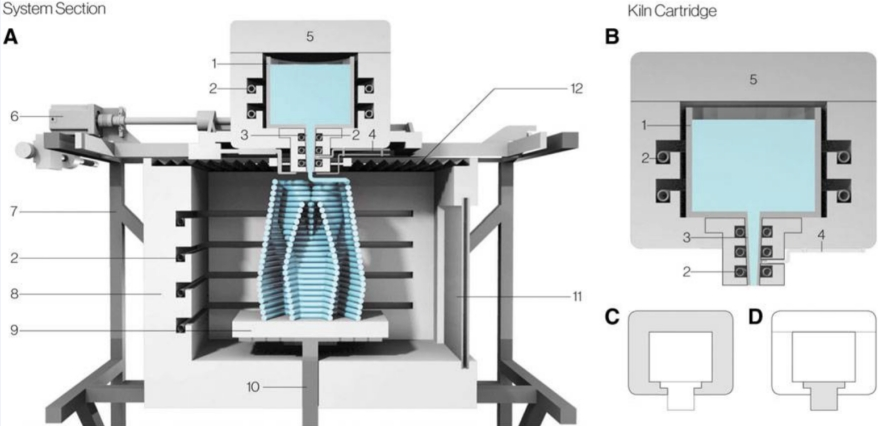
\includegraphics[width=6.4truecm]{./fig/Additive2.jpg}
  \caption{適当なサンプル2}
% \url{http://www.this.is.sample.url/} % Web上のデータの場合、参照先URLを明記
  \label{fig:ferret}
\end{figure}

\begin{figure}[H]
  \centering
  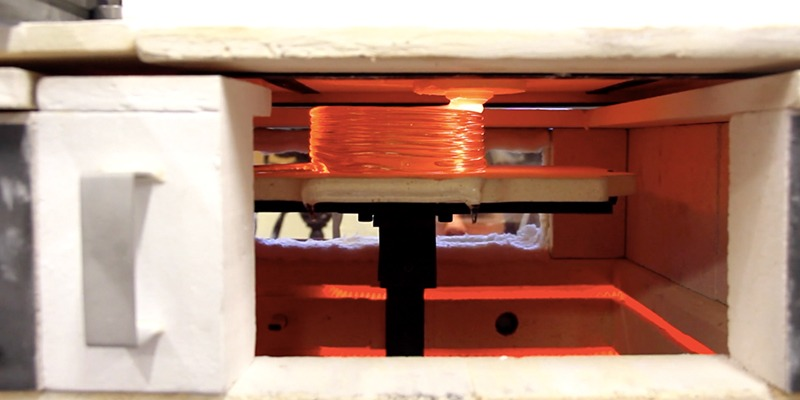
\includegraphics[width=6.4truecm]{./fig/Additive3.jpg}
  \caption{適当なサンプル2}
  \url{https://www.solidsmack.com/fabrication/mits-mediated-matter-group-unveils-transparent-glass-3d-printer/} % Web上のデータの場合、参照先URLを明記
  \label{fig:ferret}
\end{figure}

